%  A simple AAU report template.
%  2015-05-08 v. 1.2.0
%  Copyright 2010-2015 by Jesper Kjær Nielsen <jkn@es.aau.dk>
%  Modified 2023 by Andreas Højrup
%
%  This is free software: you can redistribute it and/or modify
%  it under the terms of the GNU General Public License as published by
%  the Free Software Foundation, either version 3 of the License, or
%  (at your option) any later version.
%
%  This is distributed in the hope that it will be useful,
%  but WITHOUT ANY WARRANTY; without even the implied warranty of
%  MERCHANTABILITY or FITNESS FOR A PARTICULAR PURPOSE.  See the
%  GNU General Public License for more details.
%
%  You can find the GNU General Public License 
%

%  A simple AAU report template.
%  2015-05-08 v. 1.2.0
%  Copyright 2010-2015 by Jesper Kjær Nielsen <jkn@es.aau.dk>
%  Modified 2023 by Andreas Højrup
%
%  This is free software: you can redistribute it and/or modify
%  it under the terms of the GNU General Public License as published by
%  the Free Software Foundation, either version 3 of the License, or
%  (at your option) any later version.
%
%  This is distributed in the hope that it will be useful,
%  but WITHOUT ANY WARRANTY; without even the implied warranty of
%  MERCHANTABILITY or FITNESS FOR A PARTICULAR PURPOSE.  See the
%  GNU General Public License for more details.
%
%  You can find the GNU General Public License at <http://www.gnu.org/licenses/>.
%
\documentclass[11pt, a4paper]{report}



%%%%%%%%%%%%%%%%%%%%%%%%%%%%%%%%%%%%%%%%%%%%%%%%
% Language, Encoding and Fonts
% http://en.wikibooks.org/wiki/LaTeX/Internationalization
%%%%%%%%%%%%%%%%%%%%%%%%%%%%%%%%%%%%%%%%%%%%%%%%
% Select encoding of your inputs. Depends on
% your operating system and its default input
% encoding. Typically, you should use
%   Linux  : utf8 (most modern Linux distributions)
%            latin1 
%   Windows: ansinew
%            latin1 (works in most cases)
%   Mac    : applemac
% Notice that you can manually change the input
% encoding of your files by selecting "save as"
% an select the desired input encoding. 
\usepackage[utf8]{inputenc}
% Make latex understand and use the typographic
% rules of the language used in the document.
\usepackage[danish,english]{babel}
\usepackage{csquotes}
% Use the palatino font
\usepackage[sc]{mathpazo}
\linespread{1.05}         % Palatino needs more leading (space between lines)
% Choose the font encoding
\usepackage[T1]{fontenc}
\usepackage{esvect} %included for vectors

% Used for code snippets
\usepackage{listings}

% Abbreviations

%%%%%%%%%%%%%%%%%%%%%%%%%%%%%%%%%%%%%%%%%%%%%%%%
% Graphics and Tables
% http://en.wikibooks.org/wiki/LaTeX/Importing_Graphics
% http://en.wikibooks.org/wiki/LaTeX/Tables
% http://en.wikibooks.org/wiki/LaTeX/Colors
%%%%%%%%%%%%%%%%%%%%%%%%%%%%%%%%%%%%%%%%%%%%%%%%
% load a colour package
\usepackage[table,xcdraw]{xcolor}
\definecolor{aaublue}{RGB}{33,26,82}% dark blue
% The standard graphics inclusion package
\usepackage{graphicx}
% Set the search path for \includegraphics{}
\graphicspath{./figures/}
% Set up how figure and table captions are displayed
\usepackage{caption}
\captionsetup{%
  font=footnotesize,% set font size to footnotesize
  labelfont=bf % bold label (e.g., Figure 3.2) font
}
% Make the standard latex tables look so much better
\usepackage{booktabs}
% Enable the use of frames around, e.g., theorems
% The framed package is used in the example environment
\usepackage{framed}
% Used for creating graphs and plots
\usepackage{pgfplots}
\usepgfplotslibrary{statistics}
\pgfplotsset{compat=1.18}

%For arrays
\usepackage{array}
\newcolumntype{P}[1]{>{\centering\arraybackslash}p{#1}}

%Subfigure possible
\usepackage{subcaption}



%%%%%%%%%%%%%%%%%%%%%%%%%%%%%%%%%%%%%%%%%%%%%%%%
% Mathematics
% http://en.wikibooks.org/wiki/LaTeX/Mathematics
%%%%%%%%%%%%%%%%%%%%%%%%%%%%%%%%%%%%%%%%%%%%%%%%
% Defines new environments such as equation,
% align and split 
\usepackage{amsmath}
% Adds new math symbols
\usepackage{amssymb}
% Use theorems in your document
% The ntheorem package is also used for the example environment
% When using thmmarks, amsmath must be an option as well. Otherwise \eqref doesn't work anymore.
\usepackage[framed,amsmath,thmmarks]{ntheorem}



%%%%%%%%%%%%%%%%%%%%%%%%%%%%%%%%%%%%%%%%%%%%%%%%
% Page Layout
% http://en.wikibooks.org/wiki/LaTeX/Page_Layout
%%%%%%%%%%%%%%%%%%%%%%%%%%%%%%%%%%%%%%%%%%%%%%%%
% Change margins, papersize, etc of the document
\usepackage[
  inner=28mm,% left margin on an odd page
  outer=28mm,% right margin on an odd page
  ]{geometry}
  
% Modify how \chapter, \section, etc. look
% The titlesec package is very configureable
\usepackage{titlesec}
\titleformat{\chapter}[display]{\normalfont\huge\bfseries}{\chaptertitlename\ \thechapter}{20pt}{\Huge}
\titleformat*{\section}{\normalfont\Large\bfseries}
\titleformat*{\subsection}{\normalfont\large\bfseries}
\titleformat*{\subsubsection}{\normalfont\normalsize\bfseries}
%\titleformat*{\paragraph}{\normalfont\normalsize\bfseries}
%\titleformat*{\subparagraph}{\normalfont\normalsize\bfseries}

% Clear empty pages between chapters
\let\origdoublepage\cleardoublepage
\newcommand{\clearemptydoublepage}{%
  \clearpage
  {\pagestyle{empty}\origdoublepage}%
}
\let\cleardoublepage\clearemptydoublepage

% Change the headers and footers
\usepackage{fancyhdr}
\pagestyle{fancy}
\fancyhf{} %delete everything
\renewcommand{\headrulewidth}{0pt} %remove the horizontal line in the header

%\fancyhead[RE]{\small\nouppercase\leftmark} %even page - chapter title

\fancyhead[L]{\small\nouppercase\rightmark} %uneven page - section title

\fancyhead[R]{\thepage}

% Do not stretch the content of a page. Instead,
% insert white space at the bottom of the pageretch the content of a page. Instead,
% insert white space at the bottom of the page
\raggedbottom
% Enable arithmetics with length. Useful when
% typesetting the layout.
\usepackage{calc}



%%%%%%%%%%%%%%%%%%%%%%%%%%%%%%%%%%%%%%%%%%%%%%%%
% Bibliography
% http://en.wikibooks.org/wiki/LaTeX/Bibliography_Management
%%%%%%%%%%%%%%%%%%%%%%%%%%%%%%%%%%%%%%%%%%%%%%%%
%\usepackage[backend=bibtex, bibencoding=utf8, sorting=none,]{biblatex}
\usepackage[backend=biber, bibencoding=utf8, sorting=none,]{biblatex}
%\usepackage[backend=biber,style=numeric,sortcites,natbib=true,sorting=none]{biblatex}
\addbibresource{bib/mybib.bib}



%%%%%%%%%%%%%%%%%%%%%%%%%%%%%%%%%%%%%%%%%%%%%%%%
% Misc
%%%%%%%%%%%%%%%%%%%%%%%%%%%%%%%%%%%%%%%%%%%%%%%%
% Add bibliography and index to the table of contents
\usepackage[nottoc]{tocbibind}

% Enable TODO's, added todo notes are placed in the margin of the document
%\usepackage[colorinlistoftodos,prependcaption,textsize=tiny]{todonotes}

%Can turn pages now
\usepackage{pdflscape}
\usepackage{rotating}

% Not used but was here in the original template, dont know what is was used for
%\usepackage{scrextend} % Cannot be loaded after hyperref, causes a conflict

% Used to create hyperrefs, \href, bliver brugt meget til links man gerne vil have har en anden tekst
\usepackage[hidelinks]{hyperref}
\hypersetup{%
	%pdfpagelabels=true,%
	plainpages=false,%
	pdfauthor={Author(s)},%
	pdftitle={Title},%
	pdfsubject={Subject},%
	bookmarksnumbered=true,%
	colorlinks=false,%
	citecolor=black,%
	filecolor=black,%
	linkcolor=black,% you should probably change this to black before printing
	urlcolor=black,%
	pdfstartview=FitH%
}


% Random shiet jeg ikke ved hvad gør eller bliver brugt til
\usepackage{float}
\usepackage{tabu}
\usepackage{gensymb}
\usepackage{textcomp}
\usepackage{comment, chngpage, appendix, verbatim}

\usepackage{multirow}
\usepackage{enumitem}
\usepackage[bottom]{footmisc}

\usepackage{acronym}
\usepackage[table,xcdraw]{xcolor}
\usepackage{url}
\usepackage{hyperref}
\usepackage{longtable}     

% package inclusion and set up of the document
 
%  A simple AAU report template.
%  2015-05-08 v. 1.2.0
%  Copyright 2010-2015 by Jesper Kjær Nielsen <jkn@es.aau.dk>
%  Modified 2023 by Andreas Højrup
%
%  This is free software: you can redistribute it and/or modify
%  it under the terms of the GNU General Public License as published by
%  the Free Software Foundation, either version 3 of the License, or
%  (at your option) any later version.
%
%  This is distributed in the hope that it will be useful,
%  but WITHOUT ANY WARRANTY; without even the implied warranty of
%  MERCHANTABILITY or FITNESS FOR A PARTICULAR PURPOSE.  See the
%  GNU General Public License for more details.
%
%  You can find the GNU General Public License at <http://www.gnu.org/licenses/>.
%
%
%
% see, e.g., http://en.wikibooks.org/wiki/LaTeX/Customizing_LaTeX#New_commands
% for more information on how to create macros

%%%%%%%%%%%%%%%%%%%%%%%%%%%%%%%%%%%%%%%%%%%%%%%%
% Macros for the titlepage
%%%%%%%%%%%%%%%%%%%%%%%%%%%%%%%%%%%%%%%%%%%%%%%%
%Creates the aau titlepage
\newcommand{\aautitlepage}[3]{%
  {
    %set up various length
    \ifx\titlepageleftcolumnwidth\undefined
      \newlength{\titlepageleftcolumnwidth}
      \newlength{\titlepagerightcolumnwidth}
    \fi
    \setlength{\titlepageleftcolumnwidth}{0.5\textwidth-\tabcolsep}
    \setlength{\titlepagerightcolumnwidth}{\textwidth-2\tabcolsep-\titlepageleftcolumnwidth}
    %create title page
    \thispagestyle{empty}
    \noindent%
    \begin{tabular}{@{}ll@{}}
      \parbox{\titlepageleftcolumnwidth}{
        \iflanguage{danish}{%
          
\includegraphics[width=\titlepageleftcolumnwidth]{figures/aau_logo_da}
        }{%
          
\includegraphics[width=0.9\titlepageleftcolumnwidth]{figures/aau_logo_en}
        }
      } &
      \parbox{\titlepagerightcolumnwidth}{\raggedleft\sf\small
        #2
      }\bigskip\\
       #1 &
      \parbox[t]{\titlepagerightcolumnwidth}{%
      \textbf{Abstract:}\bigskip\par
        \fbox{\parbox{\titlepagerightcolumnwidth-.15\fboxsep-2\fboxrule}{%
          #3
        }}
      }\\
    \end{tabular}
    \vfill
    \iflanguage{danish}{%
      \noindent{\footnotesize\emph{Rapportens indhold er frit tilgængeligt, men offentliggørelse (med kildeangivelse) må kun ske efter aftale med forfatterne.}}
    }{%
      \noindent{\footnotesize\emph{The content of this report is freely available, but publication (with reference) may only be pursued due to agreement with the author.}}
    }
    \clearpage
  }
}

%Create english project info
\newcommand{\englishprojectinfo}[8]{%
  \parbox[t]{\titlepageleftcolumnwidth}{
    \textbf{Title:}\\ #1\bigskip\par
    \textbf{Theme:}\\ #2\bigskip\par
    \textbf{Project Period:}\\ #3\bigskip\par
    \textbf{Project Group:}\\ #4\bigskip\par
    \textbf{Participant(s):}\\ #5\bigskip\par
    \textbf{Supervisor(s):}\\ #6\bigskip\par
    %\textbf{Copies:} #7\bigskip\par
    \textbf{Page Numbers:} \pageref{bib:mybiblio}\bigskip\par
    \textbf{Date of Completion:}\\ #8
  }
}

%Create danish project info
\newcommand{\danishprojectinfo}[8]{%
  \parbox[t]{\titlepageleftcolumnwidth}{
    \textbf{Titel:}\\ #1\bigskip\par
    \textbf{Tema:}\\ #2\bigskip\par
    \textbf{Projektperiode:}\\ #3\bigskip\par
    \textbf{Projektgruppe:}\\ #4\bigskip\par
    \textbf{Deltager(e):}\\ #5\bigskip\par
    \textbf{Vejleder(e):}\\ #6\bigskip\par
    \textbf{Oplagstal:} #7\bigskip\par
    \textbf{Sidetal:} \pageref{bib:mybiblio}\bigskip\par
    \textbf{Afleveringsdato:}\\ #8
  }
}

%%%%%%%%%%%%%%%%%%%%%%%%%%%%%%%%%%%%%%%%%%%%%%%%
% An example environment
%%%%%%%%%%%%%%%%%%%%%%%%%%%%%%%%%%%%%%%%%%%%%%%%
\theoremheaderfont{\normalfont\bfseries}
\theorembodyfont{\normalfont}
\theoremstyle{break}
\def\theoremframecommand{{\color{gray!50}\vrule width 5pt \hspace{5pt}}}
\newshadedtheorem{exa}{Example}[chapter]
\newenvironment{example}[1]{%
		\begin{exa}[#1]
}{%
		\end{exa}
}
% my new macros

\addbibresource{bib/mybib.bib}
\begin{document}

%TODO list -> Remember to un-comment in preamble
%\listoftodos[TODOs]

%frontmatter
\pagestyle{empty} %disable headers and footers
\pagenumbering{roman} %use roman page numbering in the frontmatter
%  A simple AAU report template.
%  2015-05-08 v. 1.2.0
%  Copyright 2010-2015 by Jesper Kjær Nielsen <jkn@es.aau.dk>
%  Modified 2023 by Andreas Højrup
%
%  This is free software: you can redistribute it and/or modify
%  it under the terms of the GNU General Public License as published by
%  the Free Software Foundation, either version 3 of the License, or
%  (at your option) any later version.
%
%  This is distributed in the hope that it will be useful,
%  but WITHOUT ANY WARRANTY; without even the implied warranty of
%  MERCHANTABILITY or FITNESS FOR A PARTICULAR PURPOSE.  See the
%  GNU General Public License for more details.
%
%  You can find the GNU General Public License at <http://www.gnu.org/licenses/>.
%
\pdfbookmark[0]{Front page}{label:frontpage}%
\begin{titlepage}
  \addtolength{\hoffset}{0.5\evensidemargin-0.5\oddsidemargin} %set equal margins on the frontpage - remove this line if you want default margins
  \noindent%
  \begin{tabular}{@{}p{\textwidth}@{}}
    \toprule[2pt]
    \midrule
    \vspace{0.2cm}
    \begin{center}
    \Huge{\textbf{
      Report Title% insert your title here
    }}
    \end{center}
    \begin{center}
      \Large{
        - Subtitle -% insert your subtitle here
      }
    \end{center}
    \vspace{0.2cm}\\
    \midrule
    \toprule[2pt]
  \end{tabular}
  \vspace{4 cm}
  \begin{center}
    {\large
      Project Report%Insert document type (e.g., Project Report)
    }\\
    \vspace{0.2cm}
    {\Large
      Group Name/Number%Insert your group name or real names here
    }
  \end{center}
  \vfill
  \begin{center}
  Aalborg University\\
  The Technical Faculty of IT and Design
  \end{center}
\end{titlepage}
\clearpage

\pdfbookmark[0]{English title page}{label:titlepage_en}
\aautitlepage{%
  \englishprojectinfo{
    Project Title %title
  }{%
    Scientific Theme %theme
  }{%
    Fall Semester 2025 %project period
  }{%
    1 % project group
  }{%
    %list of group members
    Anne Sofie Ingerslev\\ 
    Lærke Stein Raaschou\\
    Jonas Holm Ingvorsen\\
    Stoyan Dimitrov Mihaylov\\
    Peter Gravgaard Andersen\\
    Rasmus Mølby Nielsen
    
  }{%
    %list of supervisors
    Andreas Aakerberg 
  }{%
    1 % number of printed copies
  }{%
    \today % date of completion
  }%
}{%department and address
  \textbf{The Technical Faculty of IT and Design}\\
  Aalborg University\\
  \href{http://www.aau.dk}{http://www.aau.dk}
}{% the abstract
  Here is the abstract
 }

\cleardoublepage

\cleardoublepage
\pdfbookmark[0]{Contents}{label:contents}
\pagestyle{fancy} %enable headers and footers again

\tableofcontents
\chapter*{Preface}
\addcontentsline{Section}{Preface}
\raggedright \hfill Aalborg University \today

\vspace{3em}

\noindent Here is the preface. You should put your signatures at the end of the preface.

\vspace{3cm}
\vfill\noindent
\begin{minipage}[b]{0.45\textwidth}
 \centering
 \rule{\textwidth}{0.5pt}\\
 Anne Sofie Ingerslev \\
 {\footnotesize ainger24@student.aau.dk}
\end{minipage}
\hfill
\begin{minipage}[b]{0.45\textwidth}
 \centering
 \rule{\textwidth}{0.45pt}\\
 Lærke Stein Raaschou \\
 {\footnotesize lraasc24@student.aau.dk}
\end{minipage}
\vspace{3\baselineskip}
\begin{center}
\begin{minipage}[b]{0.45\textwidth}
 \centering
 \rule{\textwidth}{0.45pt}
 Jonas Holm Ingvorsen \\
 {\footnotesize jingvo24@student.aau.dk}
\end{minipage}
\hfill
\begin{minipage}[b]{0.45\textwidth}
 \centering
 \rule{\textwidth}{0.5pt}
 Stoyan Dimitrov Mihaylov\\
 {\footnotesize smihay24@student.aau.dk}
\end{minipage}
\end{center}
\vspace{3\baselineskip}
\begin{center}
\begin{minipage}[b]{0.45\textwidth}
 \centering
 \rule{\textwidth}{0.45pt}
 Peter Gravgaard Andersen \\
 {\footnotesize pander23@student.aau.dk}
\end{minipage}
\hfill
\begin{minipage}[b]{0.45\textwidth}
 \centering
 \rule{\textwidth}{0.45pt}
 Rasmus Mølby Nielsen \\
 {\footnotesize rmni24@student.aau.dk}
\end{minipage}
\end{center}






\begin{comment}
\begin{center}
\begin{minipage}[b]{0.45\textwidth}
 \centering
 \rule{\textwidth}{0.5pt}
 Name\\
 {\footnotesize <mail>}
\end{minipage}
\hfill
\end{center}
\end{comment}


\chapter*{Abbreviations}
A list of the abbreviations used in this report, sorted in alphabetical order:

\begin{acronym}
\acro{ReID}{Re-Identification}
\acro{POI}{Person Of Interest}
\acro{FSL}{Few-Shot Learning}
\acro{HR}{High-Resolution}
\acro{LR}{Low-Resolution}
\acro{CNN}{Convolutional Neural Network}
\acro{SR}{Super-Resolution}
\acro{POLCAM}{Police Camera Register}
\acro{IR}{Infrared}
\acro{PTZ}{Pan Tilt-Zoom}
\acro{AI}{Artificial Intelligence}
\acro{FOV}{Field Of View}
\acro{FPNN}{Filter Pairing Neural Network}
\acro{SRCNN}{Super-Resolution Convolutional Neural Network}
\acro{FFSR}{Foreground-Focus Super-Resolution}
\acro{RIFE}{Resolution-Invariant Feature-Extractor}
\end{acronym}

\cleardoublepage
%mainmatter
\pagenumbering{arabic} %use arabic page numbering in the mainmatter


%Introduction
\chapter{Introduction}
\label{cha:introduction}

Video surveillance has become a fundamental component of modern law enforcement. In Denmark, an estimated 1.5 million surveillance cameras form an extensive network that police increasingly rely upon for criminal investigations \cite{overvagningsekspert2025}. High-profile cases, such as the Emilie Meng murder investigation and the Mia Skadhauge Stevn case, demonstrate how surveillance footage can provide crucial evidence leading to breakthroughs and successful prosecutions \cite{emilie_meng_avisen, mia_stevn_avisen}.
\\\\
However, the effectiveness of surveillance systems is constrained by technical limitations. Footage frequently suffers from low resolution due to camera placement at considerable distances, hardware limitations, and challenging environmental conditions such as poor lighting and adverse weather \cite{arxiv_superres2021}. This limits the investigative value of recorded footage despite its abundance. The challenge of extracting usable information from degraded surveillance imagery represents a significant practical problem for law enforcement agencies.
\\\\
The intersection of artificial intelligence and surveillance technology presents an opportunity to address this challenge. \ac{SR} techniques, which reconstruct higher-resolution images from low-resolution observations, have advanced significantly through deep learning. When combined with person \ac{ReID} systems that track individuals across multiple camera views, these technologies offer potential to enhance investigative capabilities. This integration of computer vision techniques with real-world law enforcement needs motivated the focus of this project. 
\\\\
The proliferation of surveillance technologies also raises ethical considerations regarding privacy and civil liberties. Danish regulations, including mandatory registration through the \ac{POLCAM} and restrictions on monitoring public spaces, reflect ongoing efforts to balance security needs against fundamental rights to privacy \cite{politiet2024registrer, lov_tv_overvaagning2023}. As \ac{AI} and computer vision advance, these ethical tensions intensify, necessitating careful consideration of proportionality in system design \cite{overvagningsekspert2025, menneskeret_overvaagning}.
\\\\
This project investigates whether \ac{SR} preprocessing can improve the accuracy of person re-identification networks when applied to low-resolution surveillance imagery. The scope is deliberately focused: the project evaluates super-resolution as a preprocessing step for an existing re-identification model, measuring performance improvements on degraded surveillance footage. The project does not develop novel super-resolution or re-identification architectures, nor does it implement a complete operational system with user interfaces for deployment. Instead, the emphasis is on empirical evaluation of whether this technical approach offers practical value for law enforcement applications. Milestone Systems, a Danish surveillance software provider headquartered in Brøndby, serves as a reference point for understanding contemporary surveillance workflows, though system integration with commercial platforms falls outside the project scope \cite{MilestoneSystems2025}.
\\\\


%Problemanalysis
\chapter{Problem Analysis}
\label{cha:problemanalysis}
Before implementing a solution it is important to understand the problem of (initial problem statement). This chapter will analyze the challenges related to surveillance, focusing on both private and police usage. It explores the motivations behind surveillance and the ethical concerns that arise from their application. (når vi ved hvor Milestone skal stå, vil det også blive inkluderet)

\section{Surveillance and Surveillance Cameras: Private and Police Usage}\label{sec:police}

Camera surveillance has become a common and visible part of Danish society in the 21st century. According to estimates from SikkerhedsBranchen, around 1.5 million surveillance cameras watch over citizens' daily activities throughout Denmark \cite{overvagningsekspert2025}. This large number of cameras raises concerns about balancing security and crime prevention with privacy rights.\cite{videnskab2024}.

\subsection{Private and Commercial Motivations for Surveillance}

Private citizens install surveillance cameras mainly to protect their property from crimes like burglary and vandalism \cite{bolius2024}. The main reason is wanting to discourage potential criminals through visible cameras and warning signs \cite{bolius2024}. Also, feeling safer plays an important role and being able to see live images from home through smartphone apps gives people a sense of control and peace of mind, no matter where they are \cite{bolius2024}.
\\\\
For retail businesses and other companies, video surveillance serves multiple purposes. The primary function is preventing and investigating economic crimes, including shoplifting, employee theft, robbery, and vandalism \cite{bolius2024}. The increase in retail theft has made surveillance an essential component of store operations \cite{retailnews2025,danskerhverv2025rapport,securityuser2025}. Beyond crime prevention, surveillance is used for business analysis of customer behavior and optimizing staff resources \cite{securitas2024butik}.


\subsection{Police Usage of Surveillance Cameras}
\label{subsec:Police_Application}

Police use camera surveillance for two main purposes: preventing crime and investigating crimes that have already happened. Since 2018, Danish police have installed 450 "surveillance cameras" in public places as part of the government's security and safety package \cite{overvagningsekspert2025,videnskab2024}. These cameras are placed strategically to monitor public areas during events that might threaten public safety, such as demonstrations, high-risk football matches, and busy nightlife areas. \cite{dyhrberg2024natteliv}
\\\\
Investigating serious crimes is the most important use of these cameras. As Police Inspector Johannes Sølvsten Jönsson explains: "Materiale fra overvågningskameraer er ofte helt centralt i vores efterforskning af blandt andet grove forbrydelser som voldtægt og drab" (translated: "Material from surveillance cameras is often very important to our investigation of serious crimes such as rape and murder") \cite{politiet2024opfordrer}. Police also use other camera technologies including body-worn cameras (bodycams), which help reduce conflicts, provide strong evidence, and give objective records of police behavior. Additionally, drones help police understand complex situations during search operations and when analyzing large crime scenes.
\\\\
An important part of police surveillance strategy is \ac{POLCAM}, which works as a nationwide system for finding locations and contact information for both private and public cameras \cite{politiet2024registrer,sikkerhedsbranchen2024,securitas2024guide}. The register does not give police direct access to cameras, but allows them to quickly identify cameras that may have captured relevant footage after crimes happen \cite{politiet2024opfordrer}. This approach allows police to benefit from privately owned cameras in their investigations without investing in their own extensive camera network. 


\subsection{Preventive Effects}
\label{subsec:preventive_effects}

The idea behind surveillance as a crime prevention tool is based on rational choice theory, where visible cameras should increase the perceived risk of being caught and therefore stop potential crimes from being committing crimes. Surveillance is deeply embedded in political arguments, as shown in the government's "Security Package" \cite{tryghedspakke2019}.
\\\\
Research evidence for this preventive effect is mixed. The Danish Crime Prevention Council concludes that surveillance shows clear preventive effects only in very specific situations, mainly for property crimes in limited areas \cite{dkr_tv_overvaagning}. Research broadly agrees that surveillance has little to no preventive effect on violent crimes like assault and robbery, because these crimes often happen on impulse without careful planning \cite{videnskab2024}. This does not mean surveillance cameras lack value. Rather, their primary documented value lies in their use as investigation tools after crimes have occurred.
\\\\
In contrast, there is clear agreement about the value of video recordings as investigation tools. Recordings help police identify criminals, understand how incidents happened, clear innocent people, and provide objective evidence. Danish criminal cases demonstrate this value. In the Emilie Meng murder case from 2016, surveillance footage from Korsør Station was enhanced by specialists despite its poor quality, enabling identification of a suspect's vehicle. Combined with telecom data, this led to an arrest \cite{emilie_meng_avisen,emilie_meng_wiki}. Similarly, in the 2022 Mia Skadhauge Stevn case, surveillance cameras captured the victim entering a vehicle on Vesterbro in Aalborg, and subsequent camera footage allowed police to read the license plate, leading to a rapid breakthrough in the investigation \cite{mia_stevn_avisen}. These cases illustrate how systematic analysis of surveillance material can be crucial for investigation breakthroughs.

\subsection{Ethical Considerations}

With the number of surveillance cameras increasing, so does the risk of invading the privacy of the public \cite{overvagningsekspert2025}. Private parties are not permitted to monitor areas used for public access \cite{lov_tv_overvaagning2023} and surveillance cameras that conduct video surveillance of such an area must be registered in the \acs{POLCAM} within 14 days of installation \cite{politiet2024registrer}. 
\\\\
These registration requirements serve multiple privacy-protecting functions. First, they create transparency about where surveillance occurs, allowing citizens to be aware of monitored areas. Second, registration enables oversight authorities to verify that cameras are placed and used according to legal requirements. Third, the obligation to register discourages unauthorized surveillance of public spaces, as unregistered cameras violating the placement rules can be identified and owners held accountable \cite{kromann_polcam2021}. Together, these mechanisms help ensure that the use of cameras in public spaces remains controlled and legally compliant, thereby limiting the risk of unauthorized collection of image and video materials.
\\\\
However, new technologies such as data analysis, facial recognition and risk assessment algorithms make it difficult to preserve the right to privacy \cite{overvagningsekspert2025}. A fundamental principle in democratic surveillance is proportionality: surveillance should target specific criminal activities or individuals, not monitor the entire population to catch a few offenders. Systems that enable continuous monitoring of all citizens violate this principle and infringe upon the right to privacy, as they subject innocent people to surveillance without reasonable suspicion \cite{menneskeret_overvaagning,justitia_overvaagning}. As described in Section \ref{subsec:preventive_effects}, these new technologies are valuable tools for law enforcement. Yet, if people believe they are under constant surveillance, it will likely change their behavior in everyday life \cite{overvagningsekspert2025}. This raises the problem of balancing the value of surveillance technologies for law enforcement against the risk it poses to freedom of expression through self-censorship \cite{overvagningsekspert2025}.

\section{Milestone Systems}

Milestone Systems is a global provider of video surveillance software, headquartered in Brøndby, Denmark. Its product portfolio centers on the open-platform XProtect VMS alongside the BriefCam analytics platform and Arcules VSaaS. XProtect is trusted in 500,000+ installations worldwide and supports more than 14,000 devices, reflecting Milestone’s focus on scale and broad hardware interoperability. In public-safety contexts including law enforcement Milestone positions XProtect as the operational backbone for situational awareness, incident response, and evidence handling. BriefCam integrates tightly with XProtect and is presented by Milestone as the advanced video-analytics layer for rapid video review, real-time alerts, and deeper research/forensics (the “Review, Respond, Research” modules), with official installation and integration guidance available from Milestone’s documentation. Altogether, the Milestone BriefCam stack is widely referenced for law-enforcement workflows that compress hours of footage into actionable leads and speed up investigative timelines \cite{MilestoneSystems2025}.

\subsection{BriefCam}
As mentioned above, BriefCam is presented by Milestone as the advanced video-analytics layer tightly integrated with XProtect. In law-enforcement and public-safety workflows, BriefCam supports rapid video review, real-time alerting, and deeper investigative research through its Review, Respond, and Research modules. Of particular relevance to this report, BriefCam provides person re-identification (Re-ID) via two complementary approaches: (i) face-based matching using operator-validated watchlists, and (ii) appearance-similarity search that links visually similar individuals across non-overlapping cameras based on visual features and attributes (e.g., clothing color or carried objects). The official XProtect integration embeds these capabilities directly in the Smart Client and ties alerts and evidence handling back into XProtect’s unified management, helping compress hours of footage into actionable leads and accelerating investigative timelines \cite{MilestoneSystems2025}.



%Technical Analysis
\chapter{Technical Analysis} \label{cha: technicalanalysis}
This chapter will present and analyze the technical foundations of the problems described in Chapter \ref{cha:problemanalysis}. It focuses on surveillance equipment, computer vision techniques, person Re-Identification, image Super-Resolution, and related works.   

\section{Surveillance Equipment and Footage}
\label{subsec:Surveillance_equipment_n_footage}

Surveillance cameras are widely used in both public and private settings, and many different factors can influence the overall quality and consistency of recorded footage. Since such recordings can in some cases be the deciding factor when solving crimes, as presented in Section \ref{subsec:Police_Application}, it is important to be aware of the limitations and challenges that can occur, while also having an overall understanding of the technical structure of the systems \cite{arxiv_superres2021}.
 
\subsection{How Cameras Work}
\label{subsubsec:How_cameras_work}
Fundamentally, a camera functions by processing light and converting it into digital data. First, the light passes through a lens, which focuses it onto an image sensor that is made up of millions of photosites (pixels) that can measure the intensity of the light. These measurements are then converted into electrical signals that represent the brightness and color of the different pixels in the image \cite{unc_camera_pipeline}.
There are many underlying elements that happen as well, which can differ in each camera. For example, digital processing like white balance correction, compression and exposure adjustments are used to create the final image or video stream \cite{unc_camera_pipeline}.
An example of this process can be seen in Figure \ref{fig:camera_pipeline}.

\begin{figure}[H]
    \centering
    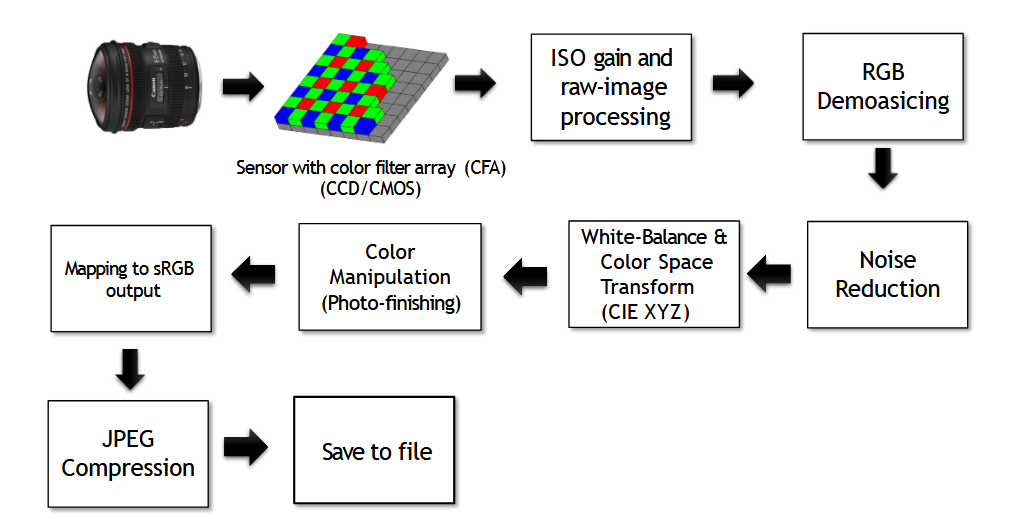
\includegraphics[width=1\linewidth]{figures/images/How_camera_works_pipeline.png}
    \caption{A typical camera pipeline.
    NOTE: This is an example for a standard consumer camera, there are many other cameras which can have different elements in it. }
    \label{fig:camera_pipeline}
\end{figure}
\noindent
These processes mostly differ from camera to camera, which all have their own distinct methods, hardware, settings and quality. This leads to differences in the final footage, an example of this can be seen in Figure \ref{fig:lens_comparison}, where images have different characteristics all depending on the camera used. It is important to understand these fundamental elements when working with surveillance recordings, as they expose the different factors that influence the final output footage, and the way it is processed and worked on \cite{korene_imatest2022_cv_iq}.
\begin{figure}[H]
    \centering
    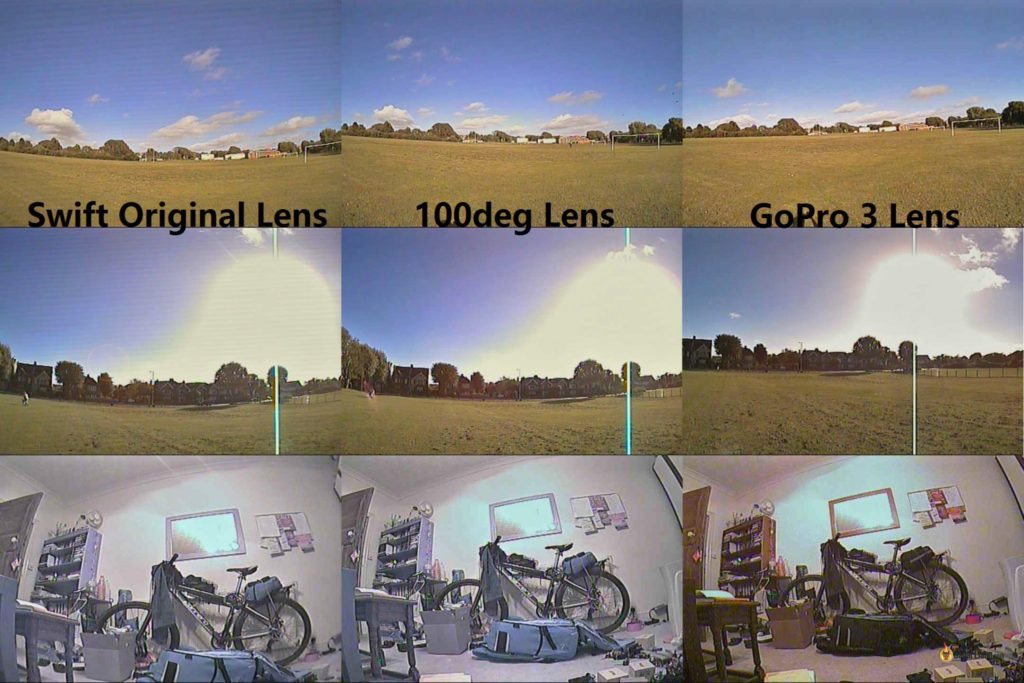
\includegraphics[width=0.7\linewidth]{figures/images/runcam-swift-lens-comparison.jpg}
    \caption{Lens comparison on different cameras to highlight change in color, brightness and \ac{FOV} in the footage.}
    \label{fig:lens_comparison}
\end{figure}
\subsection{Technical Impacts on Footage}
As stated in Section \ref{subsubsec:How_cameras_work}, there are multiple different factors that can influence the overall output of the image. The cameras themselves are rarely alike in terms of quality and features, and some have further restrictions on resolution and refresh rate to reduce energy consumption and storage, while others are able to deliver clearer images with higher resolution and smoother frame rates. In addition, certain cameras include extra functionalities such as night vision, infrared (\acs{IR}), or pan tilt-zoom (\acs{PTZ}) \cite{nightvision_enhancement2018}. This is important to be aware of when working with \ac{AI}, as computer vision works by analyzing and learning the different pixel patterns in images and videos \cite{common_challenges_image_class2024}, which, if not done correctly, can cause unwanted biases for the \acs{AI}-model when used on other surveillance systems by fixating on unimportant noise that would not be present in other instances \cite{opencv2025visionproblems}.

\subsection{Environmental Impacts on Footage}
As surveillance cameras are used for many different tasks, they will be placed in a variety of situations and conditions. Just like how the internal hardware and software can cause challenges when using \acs{AI}, the external factors such as location, season, and weather can create difficulties as well. For example, there are a lot of differences in footage from a camera that is placed inside rather than outside where weather like rain or snow can create noise which reduce clarity and usefulness in the final footage. In contrast, a camera inside is not affected by this, and therefore is viewed differently by the model \cite{arxiv_superres2021}. 
\\\\
Other aspects that can influence the models ability to generalize is light. Many surveillance cameras are used at night, where minimal visibility is achieved with a spotlight or \acf{IR} filters \cite{nightvision_enhancement2018}. However, cameras in well-lit areas have no use for these filters.
\\\\
Footage quality gets worse the greater distance it is recording. As seen in Figure \ref{fig:camera_distance}, subjects further away from the camera get blurrier and more unrecognizable, which is also one of the reasons for implementing a \acs{SR} system, that can create usable data of such cases. 
\begin{figure}[H]
    \centering
    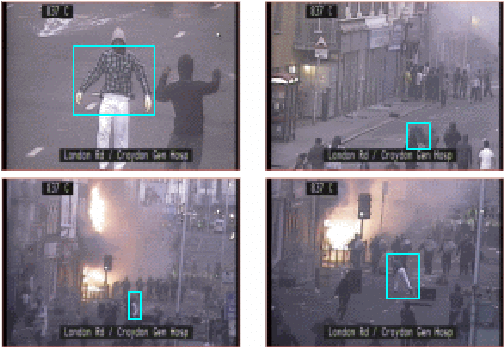
\includegraphics[width=0.7\linewidth]{figures/images/Typical-images-from-a-single-CCTV-camera-with-poor-lighting-and-long-range-camera-views.png}
    \caption{Picture from a surveillance camera in poor light and different distances to the subject marked with a cyan box.}
    \label{fig:camera_distance}
\end{figure}

\section{Computer Vision}
Denne sektion skal danne bro imellem den fysiske/kamera delen af kamera, og hvordan det omdannes til information som en maskine kan bruge. 
\\ ReID afsnittet vil senere uddybe hvordan et ReID netværk forvandler denne information til vektorer (embedding), og derfra kan genkende personer. Danner også grundlaget for at forklare forskellen på billedbaseret ReID og videobas
\\ 

\subsection{Frames as Information}
Hvad information indeholder en billedfil og hvordan indsamles/bruges denne?
\\ Lys, farver, tekstur osv. 

\subsection{Frames in a Time Series}
Hvad yderligere information kan man få fra billeder i en tidsrække? 
\\ Bevægelse, lysændringer, konsistens af objekter osv.

\section{Neural Networks}



\section{Re-identification}


\subsection{Metric Learning}


\subsection{Image-based Re-identification}


\subsection{Video-based Re-identification}


\subsection{Evaluation Metrics}


\subsection{Challenges in Surveillance Re-identification}


\section{Super-Resolution}
\label{sec:SuperResolution}

Surveillance images captured from large distances or in poor lighting conditions often result in low resolution, where important details such as facial features and clothing patterns become unclear. Super-Resolution (SR) is an image processing technique that reconstructs a High-Resolution (HR) image from one or more Low-Resolution (LR) observations, addressing the degraded imagery challenges described in Section 3.1.

The fundamental challenge with SR is that many distinct HR images can produce the same LR measurement under realistic imaging pipelines, making SR an ill-posed inverse problem without a unique solution. Practical SR systems address this by incorporating prior information about natural images to constrain the solution space \cite{Wang2019Survey,Farsiu2004Survey}. Deep learning has revolutionized SR by learning end-to-end mappings from LR to HR directly from data. The Super-Resolution Convolutional Neural Network (SRCNN) demonstrated that a compact Convolutional Neural Network (CNN) trained on bicubic downsampled pairs can outperform hand-crafted pipelines \cite{dong2015imagesuperresolutionusingdeep}.

\subsection{Downsampling vs. Real LR Images}
\label{subsec:DownsamplingVsReal}

Most academic benchmarks generate LR images by artificially downsampling HR images with bicubic interpolation, creating a domain gap between synthetic training data and real-world deployment scenarios \cite{Agustsson2017NTIRE,Timofte2017NTIRE}. Real LR images are shaped by complex degradations including optical factors (lens Modulation Transfer Function (MTF), defocus, motion blur), sensor limitations (Color Filter Array (CFA) patterns and demosaicing), and in-camera processing (tone mapping, JPEG compression). Models trained only on bicubic data often fail when confronted with these real-world degradation patterns \cite{Cai2019RealSR,Wei2020DRealSR}.

Two strategies bridge this gap. First, collecting real paired datasets like RealSR and DRealSR, which capture scenes at different resolutions and demonstrate improved transfer to real images \cite{Cai2019RealSR,Wei2020DRealSR}. Second, synthesizing realistic degradations during training, exemplified by Real-ESRGAN, which applies varying blur kernels, noise models, and compression artifacts to create diverse training data that better mimics real camera pipelines \cite{Wang2021RealESRGAN}.

Evaluation metrics depend on the test data characteristics. Peak Signal-to-Noise Ratio (PSNR) and Structural Similarity Index (SSIM) work well for bicubic benchmarks \cite{Wang2004SSIM}, while Learned Perceptual Image Patch Similarity (LPIPS) and Natural Image Quality Evaluator (NIQE) correlate better with human judgment on real-world data \cite{Zhang2018LPIPS,Mittal2013NIQE}. Best practice reports both distortion measures (PSNR/SSIM) for comparability with existing literature and perceptual assessments (LPIPS/NIQE) for practical applicability \cite{Lugmayr2020NTIRE}.

\subsection{Deep Learning Approaches}

Modern SR architectures extend early CNNs with deeper networks, residual connections, and training objectives beyond pixel-wise losses. Super-Resolution Generative Adversarial Network (SRGAN) introduced adversarial training to SR, combining a generator network with a discriminator that distinguishes real from generated images \cite{Ledig2017SRGAN}. The generator uses 16 residual blocks, while training optimizes both adversarial loss (pushing outputs toward the manifold of natural images) and perceptual loss computed in VGG-19 feature space rather than pixel space.

Enhanced SRGAN (ESRGAN) refined this approach with Residual-in-Residual Dense Blocks (RRDB) that remove batch normalization to avoid artifacts, relativistic adversarial training where the discriminator judges relative rather than absolute realism, and improved perceptual loss formulation \cite{Wang2018ESRGAN}. These refinements enabled significantly sharper textures, winning the Perceptual Image Restoration and Manipulation (PIRM) 2018 perceptual SR track.

Recent real-world variants like Real-ESRGAN incorporate the realistic degradation pipelines discussed above or employ domain adaptation techniques to improve robustness outside controlled bicubic settings \cite{Wang2021RealESRGAN,Cai2019RealSR}.

\subsection{Perception–Distortion Trade-off and Evaluation}

A central design principle for SR is the formal perception–distortion trade-off, which establishes that minimizing distortion metrics (PSNR/SSIM) while maximizing perceptual quality represents contradictory objectives that cannot be jointly optimized \cite{Blau2018PerceptionDistortion}. Methods prioritizing distortion produce smooth outputs that minimize pixel-wise error but appear blurry. Methods prioritizing perceptual quality introduce realistic high-frequency details that satisfy human observers but incur higher distortion scores.

This trade-off directly impacts application design. Forensic analysis requiring high fidelity should prioritize distortion metrics using L1/L2 losses and accept blur to avoid hallucinating details. Visual display applications should prioritize perceptual quality using adversarial and perceptual losses.

For ReID applications, this presents a critical consideration. If SR introduces perceptual improvements through hallucinated details that do not preserve discriminative features the ReID model was trained to recognize, performance may degrade despite improved visual quality. As discussed in Section 3.3.8, ReID models extract features like clothing color and coarse textures. If SR modifies these features in pursuit of perceptual realism, enhanced images may become less suitable for ReID. Comprehensive evaluation reporting both distortion measures and perceptual assessments enables informed method selection \cite{Zhang2018LPIPS,Mittal2013NIQE,Wang2004SSIM}.

\section{Super-Resolution Re-Identification}

\subsection{Trained Together or Separately}

\subsection{}


\section{Related Work - flyttes?}

\subsection{DeepReID: Deep Filter Pairing Neural Network for Person Re-Identification}

This paper proposes a \ac{FPNN} for person \ac{ReID} that automatically learns features optimal for this task directly from image data, instead of relying on hand-crafted ones \cite{FPNN}. The model uses paired filters, one set for each camera view, to learn how a person’s appearance changes across different cameras. This helps the network adapt to variations in lighting, color, angles, viewpoints, and person positions. The model learns to focus on person-specific features and becomes tolerant to imperfect detections and background clutter. 
\\\\
Despite outperforming state-of-the-art methods at the time, this solution has several limitations. The dataset used is relatively small, with 13,164 images of 1,360 different people, which may introduce bias and limit generalization. While the dataset does represent real-life scenarios of obtained data from surveillance cameras, and lighting is mentioned as a key challenge, there is no analysis of image resolution effects or how they could improve the model’s performance. This gap could be explored through integrating \ac{SR} techniques.  

\subsection{Learning a Deep Convolutional Network for Image Super-Resolution}

This paper proposes a method for single image \ac{SR} called \ac{SRCNN} \cite{SRCNN}. The method directly learns an end-to-end mapping between the low- and high-resolution images and jointly optimizes all layers to learn how to reconstruct fine details and textures from data. The mapping is implemented as a deep \ac{CNN} that takes the \ac{LR} image as the input and outputs the \ac{HR} image.
\\\\
Even though this method achieved superior performance to the state-of-the-art methods, it might not be a good idea to apply the \ac{SRCNN} to a \ac{ReID} problem. This is because \ac{SRCNN} does not know that the goal is \ac{ReID} and might distort useful features in the process of enhancing the image. An ideal \ac{SR} model for \ac{ReID} would enhance features useful for recognition, for example the edges around clothes. 	

\subsection{Resolution-invariant Person Re-Identification}

This paper proposes a method for person \ac{ReID} robust to resolution variance by jointly training a \ac{FFSR} module and a \ac{RIFE} by end-to-end \ac{CNN} learning \cite{FFSR}. \ac{FFSR} enhances the person’s image without focusing on the background. \ac{RIFE} extracts features from low- and high-resolution images through two connected streams, allowing the system to compare people’s appearance regardless of image quality. 
\\\\
Although this method is very promising in combining \ac{ReID} with \ac{SR} it does have the limitation of depending on paired low- and high-resolution images, which are unavailable in real-world settings. 


%Problem Statement
\chapter{Problem Statement} \label{cha: problemstatement}

Based on the findings in the problem analysis in Chapter \ref{cha:problemanalysis} and technical analysis in Chapter \ref{cha: technicalanalysis}, the following problem statement can be formulated:
\\

\textit{"How can a Re-identification system combined with Super-resolution be implemented as a proof-of-concept tool for law enforcement?"}

%Requirement Specifications
\chapter{Requirement Specification} 
\label{cha:reqspec}

With the before described considerations about building a \acs{ReID} system technical and ethical in Section XXX-XX.
This section will focus on, how the system is intended to operate and how it will be used, see Section \ref{sec:usecase}, which requirements this apply to it, see Section \ref{sec:reqspec}, and at last how the system will be tested to ensure the requirements is met, see Section \ref{sec:testspec}.

\section{Use Case}
\label{sec:usecase}

To better understand the intended use of a \acs{ReID} system and the resulting implications for function and design requirements, the following section presents a use case for the system. The use case is structured based on an outline from IBM \cite{usecase}.

\subsection{Re-identify a Person of Interest in New Footage}
A police officer can use the system to track a \acs{POI}, such as a thief, murderer, missing person or victim of crime, across multiple surveillance feeds once they have been found in a single video clip. The system's output can be used to map the person's route through town or locate new video sequences with greater details for an formal identification.

\vspace{1em}

\noindent\textbf{Actors}
\begin{itemize}
    \item Primary actors: Law enforcement, police investigator, security analyst.
    \item Supporting actors: Police personnel, that collects the surveillance footage from external sources, surveillance cameras.
\end{itemize}
\vspace{1em}

\noindent\textbf{Goal}

\noindent Determine whether a \acs{POI}, that already is identified in one location, is to be found in other surveillance footage in order to track the movement of the person without manually checking camera footage.

\vspace{1em}

\noindent\textbf{Preconditions}
\begin{itemize}
    \item \acs{POI} is found in one location, obtaining one or more reference photos.
    \item Data availability: New video footage has been collected from surrounding cameras by officers.
    \item The new surveillance footage has to be from same time period, insuring the \acs{POI} has the same appearance as reference photo.
    \item Ethical and legal use: The system require the actor to log in with a personal login.
    \item Ethical and legal use: The system require a case number for each use.
\end{itemize}
\vspace{1em}

\noindent\textbf{Basic flow}
\begin{enumerate}
\item  Actor uploads reference photo(-s) of \acs{POI} into the system.
\item Actor uploads camera footage into system.
\item System processes video material, selecting frames.
\item System analysis / feature extraction / improves image quality.
\item System search for match in the videos.
\item System returns list of matches over a set threshold with the video footage, to the user so they can look it through and make their verdict.
\item System saves the results and logs the use.
\end{enumerate}
\vspace{1em}

\noindent\textbf{Alternative flows}
\begin{itemize}
    \item Low confidence score on matches: The use of system is logged, a report of nothing found, and user can try with new reference photo.
\end{itemize}
\vspace{1em}

\noindent\textbf{Post conditions} 
\begin{itemize}
    \item \acs{POI} is either found on footage and the matches are returned or no conclusion.
    \item Ethical use: The use of the system is logged.
    \item Results saved for later retrieval.
\end{itemize}




\section{Requirement Specification} \label{sec:reqspec}

The scope of this project is not to implement a full functional \acs{ReID} system with all thinkable features integrated and a finished user interface. The requirement presented in this section will focus on which functionalities, performance and intended use, is expected of the system, rather than the exact design of the user face.
\\\\
The requirements are organized using MoSCoW's prioritization method, which assigns each requirement one of four priority categories; Must have, Should have, Could have and Won't have, also sometimes called Wish to have. As indicated in the name of the priority, Must have is the minimal functionalities and performance of the system, required to be functional. Should-have and Could-have are categories, that rank the less essential requirements helping to prioritize which features to focus on, when additional time becomes available. Finally, the Won't have category is for features that can't be implemented in the current iteration, but is wanted in a later iteration or the final product. 
\\
The MoSCoW method helps prioritize features by distinguishing between essential requirements and expected but less critical features \cite{Moscow}. 
\\
This project will focus on fulfilling the Must-haves and, the amount of Should-haves the time constraint allows.
\\\\
The requirements are divided into three separate tables, describing the three types of requirements: Model, Usage and Safety, providing structure and clarifying which aspect the requirement addresses. Furthermore, two categories are added to the description of the requirements; functional or non-functional. This category states if the requirement specifies a functionality of the system or how well it should perform. The tables has a column called Traceability, which states which section the requirement originates from.

\begin{table}[H]
\begin{tabular}{|>{\raggedright\arraybackslash}p{0.1\linewidth}|>{\raggedright\arraybackslash}p{0.3\linewidth}|>{\raggedright\arraybackslash}p{0.15\linewidth}|>{\raggedright\arraybackslash}p{0.15\linewidth}|>{\raggedright\arraybackslash}p{0.15\linewidth}|}\hline
\rowcolor[HTML]{D8E9F7} 
\textbf{Req. nr}& \textbf{Model Requirements} & \textbf{Priority}                                        & \textbf{Category}                 & \textbf{Traceability}              \\\hline
 1& The system correctly identifies a person in at least X\% of test cases. // The system has an accuracy (precision/recall or F1 score) of at least xxx\%. & \cellcolor[HTML]{E0FFCC} Must have& \cellcolor[HTML]{FFECF5}Non-functional&\\\hline
 2& The system connects to the police login database to authenticate users.& \cellcolor[HTML]{FEFFD6} Should have& \cellcolor[HTML]{EBE4F7}Functional&\\\hline
 3& The system connects to the police case database to authenticate case reference.& \cellcolor[HTML]{FEFFD6} Should have& \cellcolor[HTML]{EBE4F7}Functional&\\ \hline
 4& The system has a web-based graphical user interface accessible through a standard browser.& \cellcolor[HTML]{E0FFCC} Must have& \cellcolor[HTML]{EBE4F7}Functional&\\\hline\end{tabular}
\end{table}

\begin{longtable}{|>{\raggedright\arraybackslash}p{0.1\linewidth}
                        |>{\raggedright\arraybackslash}p{0.3\linewidth}
                        |>{\raggedright\arraybackslash}p{0.15\linewidth}
                        |>{\raggedright\arraybackslash}p{0.15\linewidth}
                        |>{\raggedright\arraybackslash}p{0.15\linewidth}|}\hline
\rowcolor[HTML]{D8E9F7} \cellcolor[HTML]{D8E9F7}
\textbf{Req. nr}& \textbf{Usage Requirements} & \textbf{Priority} & \textbf{Category} & \textbf{Traceability} \\\hline
 5& The system allows the user to upload one query image.& \cellcolor[HTML]{E0FFCC} Must have& \cellcolor[HTML]{EBE4F7}Functional&\\\hline
 6& The system allows the user to upload multiple query images.& \cellcolor[HTML]{FFE7D1}Could have& \cellcolor[HTML]{EBE4F7}Functional&\\\hline
 7& The system allows the user to upload one frame sequence to gallery.& \cellcolor[HTML]{E0FFCC} Must have& \cellcolor[HTML]{EBE4F7}Functional&\\\hline
 8& The system allows the user to upload multiple frame sequences to gallery.& \cellcolor[HTML]{FEFFD6} Should have& \cellcolor[HTML]{EBE4F7}Functional&\\\hline
 9& The system allows the user to upload video format to gallery.& \cellcolor[HTML]{F4C1C1} Won't have& \cellcolor[HTML]{EBE4F7}Functional&\\\hline
 10& The system allows the user decide the order forwhich the system analyze the material.& \cellcolor[HTML]{FFE7D1}Could have& \cellcolor[HTML]{EBE4F7}Functional&\\\hline
 11& The system prioritizes the order of video analysis based on geotags.
The prioritization is determined by the geographical distance between each video’s geotag and the geotag of the reference photo.
Videos closer to the reference photo location shall be analyzed first.& \cellcolor[HTML]{F4C1C1} Won't have& \cellcolor[HTML]{EBE4F7}Functional&\\\hline
 12& The system returns a list of matches, when all material is analyzed.& \cellcolor[HTML]{E0FFCC} Must have& \cellcolor[HTML]{EBE4F7}Functional&\\\hline
 13& The system returns intermediate results whenever a match is found, before finishing the full analysis.& \cellcolor[HTML]{FFE7D1}Could have& \cellcolor[HTML]{EBE4F7}Functional&\\\hline
 14& The system provide a confidence score for each detected match, and only return results above a configurable threshold.& \cellcolor[HTML]{E0FFCC} Must have& \cellcolor[HTML]{FFECF5}Non-functional&\\\hline
 15& For each match, the system returns camera ID and timestamp of the frame or video.& \cellcolor[HTML]{E0FFCC} Must have& \cellcolor[HTML]{EBE4F7}Functional&\\\hline
 16& The system returns the relevant frame for which a match is detected.& \cellcolor[HTML]{FEFFD6} Should have& \cellcolor[HTML]{EBE4F7}Functional&\\\hline
 17& The system returns relevant video footage for each match.& \cellcolor[HTML]{F4C1C1} Won't have& \cellcolor[HTML]{EBE4F7}Functional&\\\hline 
\end{longtable}

\begin{table}[H]
\begin{tabular}{|>{\raggedright\arraybackslash}p{0.1\linewidth}|>{\raggedright\arraybackslash}p{0.3\linewidth}|>{\raggedright\arraybackslash}p{0.15\linewidth}|>{\raggedright\arraybackslash}p{0.15\linewidth}|>{\raggedright\arraybackslash}p{0.15\linewidth}|}\hline
\rowcolor[HTML]{D8E9F7} 
\textbf{Req. nr}& \textbf{Safety Requirements} & \textbf{Priority}                                        & \textbf{Category}                 & \textbf{Traceability}              \\\hline
        18&                    The system requires user authentication with a valid login before access is granted& \cellcolor[HTML]{E0FFCC} Must have& \cellcolor[HTML]{FFECF5}Non-functional& \\\hline19& The system shall require a valid case number to be entered before any analysis can be performed.& \cellcolor[HTML]{E0FFCC} Must have& \cellcolor[HTML]{FFECF5}Non-functional&\\\hline
        20&                    The system logs each use of the system, including: User ID, Timestamp, case number, attached files and results.& \cellcolor[HTML]{E0FFCC} Must have& \cellcolor[HTML]{FFECF5}Non-functional& \\\hline\end{tabular}
\end{table}

\section{Test Specification}
\label{sec:testspec}

In order to check if all requirements from Section \ref{sec:reqspec} are met and implemented properly, this section will present a test specification, as a plan for how each requirement for the system is tested. For each requirement one or more test cases are defined, specifying an input and the expected result for a given scenario under a defined set of conditions. This ensures a clear definition for when a requirement is fulfilled: if the result of the test case matches the expected outcome, the requirement is met, otherwise, the system has to be modified \cite{testspec_geek}.

\section{Test cases}
The test cases presented in this section are designed to verify whether the requirements of the system are met. Since it is expected that the final system only will fulfill the requirements prioritized \textit{must have} or \textit{should have}, the test cases is limited to these requirements. 
For each test case, one or more requirement ID's are referenced to ensure clarity and traceability. Furthermore, each test case is structured with test case ID, input and expected result.\vspace{1em}

\noindent \hrulefill

\vspace{1em}
\noindent\textbf{Test case ID: 2}
\vspace{1em}

\noindent Req. nr. 2
\vspace{1em}

\noindent Description: 
Verify that the system connects to the police login database to authenticate users.\\
\vspace{1em}

\noindent Precondition:
\begin{itemize}
    \item A valid user account exist in database
\end{itemize}
\vspace{1em}

\noindent Input:
\begin{itemize}
    \item Username: valid\_officer
    \item Password: correctPassword321
\end{itemize}
\vspace{1em}

\noindent Expected output:
\begin{itemize}
    \item     The system successfully connects to the police login database.
    \item The user is authenticated and granted access to the system.
\end{itemize}
\vspace{1em}

\noindent Post conditions:
\begin{itemize}
    \item User can use the system
\end{itemize}

 \noindent \hrulefill




Der skal skrives test cases til:

R 1: The system correctly identifies a person in at least X\% of test cases. // The system has an accuracy (precision/recall or F1 score) of at least xxx\%. 

R 2:	The system connects to the police login database to authenticate users.

R 3:	The system connects to the police case database to authenticate case reference.

R 4:	The system has a web-based graphical user interface accessible through a standard browser.

R 5:	The system allows the user to upload one query image.

R 6:	The system allows the user to upload multiple query images.

R 7:	The system allows the user to upload one frame sequence to gallery.

R 8:	The system allows the user to upload multiple frame sequences to gallery.

R 12:	The system returns a list of matches, when all material is analyzed.	

R 14: The system provide a confidence score for each detected match, and only return results above a configurable threshold.

R 15:	For each match, the system returns camera ID and timestamp of the frame or video.

R 16:	The system returns the relevant frame for which a match is detected.

R 18: The system requires user authentication with a valid login before access is granted

R 19: The system shall require a valid case number to be entered before any analysis can be performed.

R 20: The system logs each use of the system, including: User ID, Timestamp, case number, attached files and results.



INFORMATION TIL TESTCASE OPBYGNING
\begin{itemize}
    \item \textbf{Test Objectives: }Specifies the goals of each test while defining what aspects of the software are being evaluated.
    \item \textbf{Test Scope:} The specific features, functionalities, or modules covered within the testing process.
    \item \textbf{Test Scenarios:} A list of use cases and potential situations that testers will simulate during the evaluation.
    \item \textbf{Test Data:} The specific data sets required to execute each test scenario.
    \item \textbf{Expected Results:} The anticipated outcomes for each test case, providing a clear benchmark for success.
    \item \textbf{Pass/Fail Criteria:} The defined set of parameters that determine whether a test is a pass or fail. This helps ensure objectivity in the evaluation process.
    \item \textbf{Test Procedures:} Step-by-step instructions detailing how to execute each test case, promoting consistency and clarity for testers.
\end{itemize}


\begin{itemize}
    \item \textbf{Maintain Traceability:} Establish a clear link between test cases and specific software requirements. This helps enable easy identification of the functionalities during evaluation.
    \item \textbf{Prioritize Test Cases:} Not all tests are equal. Emphasize test cases based on risk assessment and application criticality. This ensures focus on areas with the highest potential for defects.
\end{itemize}

https://autify.com/blog/software-test-specification-a-step-toward-flawless-functionality


%Dataanalysis
\chapter{Data Analysis} \label{cha: data}

%Implementation
\chapter{Implementation} \label{cha: implementation}

%Methods
\chapter{Methods} \label{cha: methods}


%Discussion
\chapter{Discussion} \label{cha: discussion}

%Conklusion
\chapter{Conclusion} \label{cha:conclusion}
Here we conclude things and the chapter number is \ref{cha:conclusion}.\\



%Bibliography
% \printbibliography[heading=bibintoc]
%\bibliographystyle{IEEEtran}
%\bibliography{bib/mybib}

\label{bib:mybiblio}

%Appendix
\cleardoublepage
\pagenumbering{alph} % If appendix is more than 27 pages use {roman}
\appendix
\chapter{Appendix}\label{cha:appendix}

\subsection{Use of AI}
In carrying out the project, both in developing the system and in documenting the implementation and results, generative AI has been used. Multiple large language models, LLMs have been used for various aspects during the project, including ChatGPT, Claude, Perplexity, Gemini and CoPilot. The use of a specific model depends on individual preferences and applications.
\\
During documentation of the project, generative AI have been useful in correcting language, ensuring that the message come across clearly. LLMs is excellent at repetitive task such as formatting data. When applied to such tasks, the outputs have been reviewed afterward to make sure nothing is altered. Furthermore, LLMs have been used when setting up layout in LaTeX as well as correcting LaTeX errors. Finally, LLM has been used to summarize and presenting methods, giving a preunderstanding to a subject before further reading.
\\
In developing the AI system, generative AI have mostly been used for debugging. Some error messages are difficult to decode. Generative AI can not only simplify the problem but also assist with code changes to solve the problem. This drastically reduces the time spend on debugging, allowing for time spend on improving model and testing different configurations. In addition, Generative AI has been used for a quick documentation description, examples of application of methods and brainstorming alternative solutions. 


\end{document}